\documentclass[11pt,a4paper]{article}

% ============================================================
% Standard English mathematical typesetting preamble
% ============================================================
\usepackage[utf8]{inputenc}
\usepackage[T1]{fontenc}
\usepackage[english]{babel}
\usepackage{amsmath,amssymb,amsthm}
\usepackage{geometry}
\geometry{margin=1in}
\usepackage{booktabs}
\usepackage{array}
\usepackage{fancyhdr}
\usepackage{titlesec}
\usepackage{enumitem}
\usepackage{mathtools}
\usepackage{bm}
\usepackage{tikz}

% Theorem-like environments
\theoremstyle{plain}
\newtheorem{theorem}{Theorem}
\newtheorem{lemma}{Lemma}
\theoremstyle{definition}
\newtheorem{remark}{Remark}

% Page style
\pagestyle{fancy}
\fancyhf{}
\fancyhead[C]{\small Cayley --- Collected Mathematical Papers, Vol.\ VIII}
\fancyfoot[C]{\thepage}
\renewcommand{\headrulewidth}{0.4pt}

% Section formatting
\titleformat{\section}{\large\scshape\centering}{}{0em}{}
\titleformat{\subsection}{\normalsize\bfseries}{}{0em}{}

% Custom commands
\newcommand{\dd}{\,d}
\newcommand{\cosec}{\operatorname{cosec}}

\begin{document}

% ============================================================
% PAPER 531 (continuation: ``Smith's Prize'' Papers; Solutions)
% Book pages 442--457
% ============================================================
\section*{[531] A ``Smith's Prize'' Paper; Solutions \textnormal{(continued)}}

\bigskip
\textit{p.~442 [531]}
\smallskip

\noindent
where $\dfrac{d\xi}{dt}$, $\dfrac{d\eta}{dt}$ are the velocities of the ball and cannon respectively at the instant of
emergence; $\int_0^t \phi(x+S)(v+dS)$, is a constant factor in a quantity independent of the weights of the ball and cannon), and putting it $=\tfrac{1}{2}V$, the equation may be written
\[
(v+V)^2 = \left(\tfrac{1}{m}+\tfrac{1}{M}\right)C,
\]
where $v$, $V$ are the velocities at the moment of emergence.

But from the equation
\[
m\frac{d^2x}{dt^2} = M\frac{d^2X}{dt^2},
\]
(the initial values of the velocities being each $=0$), we have
\[
mv = MV;
\]
and hence from the foregoing equation we obtain
\[
v = \frac{M}{M+m}(V+v)
  = \frac{M}{M+m}\frac{\sqrt{(M+m)C}}{\sqrt{Mm}}
  = \frac{\sqrt{M}}{\sqrt{m}\sqrt{M+m}}\sqrt{C}
  = \frac{\sqrt{C}}{\sqrt{m}\sqrt{\left(1+\frac{m}{M}\right)}},
\]
or say
\[
v\sqrt{m} = \frac{\sqrt{C}}{\sqrt{\left(1+\frac{m}{M}\right)}}.
\]

And similarly for the other cannon, if $m_1$, $M_1$ be the masses of the ball and cannon,
$v_1$ the velocity of the ball, we have
\[
v_1 \sqrt{m_1} = \frac{\sqrt{C}}{\sqrt{\left(1+\frac{m_1}{M_1}\right)}},
\]
whence
\[
v\sqrt{m} : v_1 \sqrt{m_1} = \sqrt{\left(1+\frac{m_1}{M_1}\right)} : \sqrt{\left(1+\frac{m}{M}\right)}.
\]

If $m_1 = m$, $M_1 = \alpha$, then $v$, $v_1$ may be taken to be the velocities of the same ball fired
from the cannon, mass $M$, when it is free to recoil and when it is absolutely fixed;
and we have
\[
v : v_1 = 1 : \sqrt{\left(1+\frac{m}{M}\right)},
\]
viz.\ the velocity in the former case is equal to that in the latter case divided by
\[
\sqrt{\left(1+\frac{m}{M}\right)}.
\]

\clearpage

\bigskip
\textit{p.~443 [531]}
\smallskip

4.\ \textit{If $X : Y : Z = \eta\zeta' - \eta'\zeta : \zeta\xi' - \zeta'\xi : \xi\eta' - \xi'\eta$, where $\xi^2+\eta^2+\zeta^2=0$, $\xi'^2+\eta'^2+\zeta'^2=0$, show that $\xi\xi'$, $\eta\eta'$, $\zeta\zeta'$, $\eta\zeta' + \eta'\zeta$, $\zeta\xi' + \zeta'\xi$, $\xi\eta' + \xi'\eta$ are proportional to quadric functions of $X$, $Y$, $Z$.}

We have
\begin{align*}
Y^2 + Z^2 &= (\zeta\xi' - \zeta'\xi)^2 + (\xi\eta' - \xi'\eta)^2 \\
          &= \xi'^2(\eta^2+\zeta^2) + \xi^2(\eta'^2+\zeta'^2)
             -2\xi\xi'(\eta\eta'+\zeta\zeta')
\end{align*}
which, in virtue of the equations
\[
\xi^2 + \eta^2 + \zeta^2 = 0, \quad \xi'^2 + \eta'^2 + \zeta'^2 = 0,
\]
is
\begin{align*}
&= -2\xi^2\xi'^2 -2\xi\xi'(\eta\eta' + \zeta\zeta')\\
&= -2\xi\xi'(\xi\xi' + \eta\eta' + \zeta\zeta').
\end{align*}

And again
\begin{align*}
YZ &= (\zeta\xi' - \zeta'\xi)(\xi\eta' - \xi'\eta) \\
   &= \xi\xi'(\eta\zeta' + \eta'\zeta) - \xi'^2\eta\zeta - \xi^2\eta'\zeta',
\end{align*}
which, in virtue of the same equations, is
\begin{align*}
&= \xi\xi'(\eta\zeta' + \eta'\zeta)
   + \eta\zeta(\eta'^2+\zeta'^2)+\eta'\zeta'(\eta^2+\zeta^2)\\
&= (\eta\zeta' + \eta'\zeta)(\xi\xi' + \eta\eta' + \zeta\zeta'),
\end{align*}
and, forming the analogous equations by symmetry, the factor $(\xi\xi' + \eta\eta' + \zeta\zeta')$ divides
out, and we have
\begin{align*}
&Y^2+Z^2 : Z^2+X^2 : X^2+Y^2 : -2YZ : -2ZX : -2XY\\
&\qquad= \xi\xi' : \eta\eta' : \zeta\zeta' : \eta\zeta'+\eta'\zeta :
\zeta\xi'+\zeta'\xi : \xi\eta'+\xi'\eta,
\end{align*}
which is the required theorem.

5.\ \textit{Two tangents of a conic are harmonically related to a second conic; find the locus of the intersection of the two tangents.}

\textit{In plane geometry the angle in a semicircle is, in spherical geometry it is not, a right angle: show how these conclusions follow from the solution of the above problem.}

Let the equation of the first conic be $x^2 + y^2 + z^2 = 0$; its equation in line
coordinates is therefore $u^2+v^2+w^2=0$; or what is the same thing, the line
$ux + vy + wz = 0$ will be a tangent of the conic if only $u^2 + v^2 + w^2 = 0$.
Hence the equations of the two tangents being
\[
\xi x + \eta y + \zeta z = 0,
\]
\[
\xi' x + \eta' y + \zeta' z = 0,
\]
we have $\xi^2 + \eta^2 + \zeta^2 = 0$, $\xi'^2 + \eta'^2 + \zeta'^2 = 0$, and $X$, $Y$, $Z$ the coordinates of
the point of intersection of these tangents, we have
\[
X : Y : Z = \eta\zeta' - \eta'\zeta : \zeta\xi' - \zeta'\xi : \xi\eta' - \xi'\eta,
\]

\hfill 56---2

\clearpage

\bigskip
\textit{p.~444 [531]}
\smallskip

and thence, by the last question,
\[
\xi\xi' : \eta\eta' : \zeta\zeta' : \eta\zeta' + \eta'\zeta : \zeta\xi' + \zeta'\xi : \xi\eta' + \xi'\eta
\]
\[
= Y^2 + Z^2 : Z^2 + X^2 : X^2 + Y^2 : -2YZ : -2ZX : -2XY.
\]

Suppose that the equation of the second conic in line coordinates is
\[
(a, b, c, f, g, h)(u, v, w)^2 = 0,
\]
the condition in order that the two lines $\xi x + \eta y + \zeta z = 0$, $\xi' x + \eta' y + \zeta' z = 0$, may be
harmonically related to this conic is
\[
(a, b, c, f, g, h)(\xi, \eta, \zeta)(\xi', \eta', \zeta') = 0;
\]
or, what is the same thing, it is
\[
a\xi\xi' + b\eta\eta' + c\zeta\zeta'
+ f(\eta\zeta' + \eta'\zeta)
+ g(\zeta\xi' + \zeta'\xi)
+ h(\xi\eta' + \xi'\eta)=0,
\]
or, substituting the proportional quadric functions found above,
\[
a(Y^2+Z^2)+b(Z^2+X^2)+c(X^2+Y^2)-2fYZ-2gZX-2hXY=0,
\]
or, what is the same thing,
\[
(a + b + c)(X^2 + Y^2 + Z^2) - (a, b, c, f, g, h)(X, Y, Z)^2 = 0,
\]
as the locus of the point of intersection of the two conics; the required locus is therefore a conic.

It is to be observed that the locus is that of a point which is such that the
pairs of tangents from it to the two given conics respectively form a harmonic pencil;
viz.\ if the equations of the given conics (in line coordinates) are
\[
u^2 + v^2 + w^2 = 0,
\]
\[
(a, b, c, f, g, h)(u, v, w)^2 = 0;
\]
then the equation of the required locus, or say the equation of the harmonic conic, is
(in point coordinates)
\[
(a + b + c)(x^2 + y^2 + z^2) - (a, b, c, f, g, h)(x, y, z)^2 = 0.
\]

In particular, if the second conic be a point-pair or, say, if its equation be
\[
(\alpha u + \beta v + \gamma w)(\alpha' u + \beta' v + \gamma' w) = 0,
\]
then the equation of the harmonic conic is
\[
(\alpha\alpha' + \beta\beta' + \gamma\gamma')(x^2 + y^2 + z^2) = (\alpha x + \beta y + \gamma z)(\alpha' x + \beta' y + \gamma' z),
\]
which is satisfied by writing $(x, y, z) = (\alpha, \beta, \gamma)$, or $= (\alpha', \beta', \gamma')$, viz.\ the harmonic
conic passes through the two points of the point-pair. And so, if the first conic be
a point-pair, the harmonic conic passes through the four points of the two point-pairs.

\clearpage

\bigskip
\textit{p.~445 [531]}
\smallskip

The equation of the first conic in point coordinates is $x^2 + y^2 + z^2 = 0$; hence,
supposing as above, that the second conic is a point-pair, the intersections of the first
conic with the harmonic conic are given by
\[
x^2 + y^2 + z^2 = 0, \quad (\alpha x + \beta y + \gamma z)(\alpha' x + \beta' y + \gamma' z) = 0;
\]
whence the harmonic conic has double contact with the first conic, only if each of
the lines $\alpha x + \beta y + \gamma z$, $\alpha' x + \beta' y + \gamma' z = 0$, touches the first conic; or, what is the same
thing, if each of the points $(\alpha, \beta, \gamma)$, $(\alpha', \beta', \gamma')$ lies on the first conic.

In plane geometry, we have (in the plane) a point-pair, the two circular points
at infinity; any conic through these points is a circle: the two lines harmonic in
regard hereto are at right angles. Hence, by what precedes, taking one of the given
conics to be the circular points at infinity, and the other conic to be any two points
$P$, $Q$; the locus of the intersection of lines through $P$, $Q$, cutting each other at right
angles, is a circle; this is evidently the circle standing on $PQ$ as diameter, or the
angle in a semicircle is a right angle.

In spherical geometry we have (on the sphere) an imaginary conic $x^2 + y^2 + z^2 = 0$,
called the \textit{absolute}; any conic having double contact herewith is a circle (small circle
of the sphere); two lines (arcs of great circles), harmonic in regard hereto, are at right
angles. Hence, taking one of the conics to be the conic $x^2 + y^2 + z^2 = 0$ and the other
to be the two points $P$, $Q$; the locus of the intersections of the lines (arcs of great
circles) through $P$, $Q$, which cut at right angles, is a spherical conic; but it is not a
circle unless the points $P$, $Q$, are each of them on the conic $x^2 + y^2 + z^2 = 0$, viz.\ it is
not a circle for any two real points whatever; that is, in spherical geometry, the
angle in a semicircle is not a right angle.

\medskip
\noindent
6.\ \textit{A mass $M$ attached to the end $A$ of a chain $AC$ is placed (with the chain)
on a horizontal plane, in such wise that a portion $AB$ of the chain forms a straight
line, the remaining portion $BC$ being heaped up at $B$: the mass $M$ is then set in
motion in the direction $B$ to $A$ with a given velocity, and so moves in a straight line,
dragging the chain: determine the motion; and explain the peculiarity of the dynamical
problem.}

\medskip

The mass attached to the end of the chain is taken to be $M$, and the mass of
a unit of length of the chain to be $=m$; suppose also that at the commencement
of the motion the distance $CA$ is $=a$, and that at the end of the time $t$ this distance
is $=a+x$, so that the length of chain then in motion is $=a+x$, ($a < l - a$, if $l$ be
the whole length of the chain). Suppose also that the velocity at the time $t$ is $=v$;
then we have a mass $=M+m(a+x)$ moving with a velocity $v$; and, in the element
of time $dt$, this sets in motion with the velocity $v$ a length of chain $dx = vdt$, or mass
of chain $= mvdt$; if then the impulse backwards on the mass $M+m(a+x)$, and
forwards on the element $mvdt$ be $=R$, we have
\[
\{M+m(a+x)\}\dd v = -R,
\]
\[
mvdt \cdot v = R,
\]

\clearpage

\bigskip
\textit{p.~446 [531]}
\smallskip

that is,
\[
[M+m(a+x)]\,dv + mv^2dt = 0;
\]
or, observing that $vdt = dx$, this may be written
\[
(M+ma)\,dv + m\,d.xv = 0,
\]
that is,
\[
[M+m(a+x)]v = \text{constant},
\]
\[
= (M+ma)V,
\]
if $V$ be the velocity at the commencement of the motion. The equation gives, in
terms of the space $x$, the velocity $v$ at any time $t$ before the whole chain is set in
motion; writing it in the form
\[
\{M+m(a+x)\}\frac{dx}{dt} = (M+ma)V,
\]
we have
\[
(M+ma)x+\tfrac{1}{2}mx^2 = (M+ma)Vt,
\]
and putting herein $x = l - a$, the equation gives the value of $t$ at the instant when
the whole chain is set in motion; after this epoch, the mass and chain will (it is
clear) move on with a uniform velocity
\[
= \frac{(M+ma)V}{M+ml},
\]
The foregoing equation
\[
[M+m(a+x)]v = (M+ma)V
\]
might have been obtained at once by the consideration that the momentum is constant
throughout the motion; but the method employed puts more clearly in evidence the
peculiarity of the dynamical problem; viz.\ it is, so to speak, a problem of continuous
impulse: in each element of time $dt$ an infinitesimal element of mass has its velocity
abruptly altered (in the present problem from $0$ to $v$), but, for the very reason that
it is an infinitesimal element of mass which undergoes this abrupt change of velocity,
the effect is a continuous, not an abrupt, change of velocity of the whole finite mass
which is then in motion.

\medskip
\noindent
7.\ \textit{Show how an ellipse may be constructed as the envelope of a variable circle
having its centre upon either of the axes; and examine the geometrical peculiarities which
occur according as the major or the minor axis is made use of.}

\medskip
Considering the ellipse
\[
\frac{x^2}{a^2} + \frac{y^2}{b^2} = 1,
\]
the equation
\[
(x - \alpha)^2 + y^2 = \gamma^2,
\]
where $\alpha$ and $\gamma$ are in the first instance arbitrary parameters, represents a circle having
its centre on the major axis: in order that this may touch the ellipse, a relation
must be established between $\alpha$ and $\gamma$. When this is done we obtain a variable circle

\clearpage

\bigskip
\textit{p.~447 [531]}
\smallskip

(the equation of which contains a single arbitrary parameter), and this circle has the
ellipse for its envelope. (On account of the symmetry in regard to the axis of $x$, the
circle will, it is clear, touch the ellipse in two points, situate symmetrically in regard
to this axis.) Now to make the circle touch the ellipse, eliminating $y$, we have
\[
(x - \alpha)^2 + b^2\left(1 - \frac{x^2}{a^2}\right) - \gamma^2 = 0,
\]
that is,
\[
x^2\left(1 - \frac{b^2}{a^2}\right) - 2\alpha x + \alpha^2 + b^2 - \gamma^2 = 0,
\]
which equation, considered as an equation in $x$, must have equal roots; that is, we
must have
\[
\left(1 - \frac{b^2}{a^2}\right)(\alpha^2 + b^2 - \gamma^2) - \alpha^2 = 0;
\]
or, what is the same thing,
\[
-b^2\alpha^2 + (a^2-b^2)(b^2-\gamma^2) = 0;
\]
consequently
\[
\gamma^2 = b^2\left(1 - \frac{\alpha^2}{a^2 - b^2}\right);
\]
or the required equation of the circle is
\[
(x - \alpha)^2 + y^2 = b^2\left(1 - \frac{\alpha^2}{a^2 - b^2}\right);
\]
or, as this may also be written
\[
(x - \alpha)^2 + y^2 = (1 - e^2)\left(\frac{a^2}{e^2} - \alpha^2\right);
\]

It is to be observed that at the points of contact of the ellipse and circle, we have
\[
x = \frac{a^2}{a^2 - b^2}\alpha = \frac{\alpha}{e^2}.
\]
By simply interchanging $a$ and $b$, it appears that when the centre is on the minor axis,
the equation of the variable circle is
\[
x^2 + (y - \beta)^2 = b^2\left(1 - \frac{\beta^2}{b^2 - a^2}\right);
\]
and that at the points of contact of the ellipse and circle we have
\[
y = \frac{b^2}{b^2 - a^2}\beta.
\]

In the case where the point is on the major axis, then attending to positive
values of $\alpha$, the circle remains real so long as $\alpha$ is $< ae$, but if $\alpha$ is $=ae$, that is,
if the centre be at the focus, the radius of the circle is $=0$. But from the formula
$x = \alpha/e^2$, we have $x = a$ for $\alpha = ae^2$ and, when $\alpha$ becomes greater than this, the points
of contact are imaginary. That is, as $\alpha$ passes from $0$ to $ae^2$, the circle is real, and

\clearpage

\bigskip
\textit{p.~448 [531]}
\smallskip

has real contact with the ellipse; for $\alpha = ae^2$ the circle becomes the circle of maximum
curvature, touching the ellipse at the extremity of the major axis; as $\alpha$ increases from
$ae^2$ to $ae$, the circle is still real but its contact with the ellipse is imaginary; for
$\alpha = ae$, the circle reduces itself to the focus considered as an evanescent circle; and
for greater values of $\alpha$, the circle is imaginary.

When the centre is on the minor axis it appears in like manner that the circle
is always real; but, attending to negative values of $\beta$, the circle has real contact
with the ellipse only so long as $\beta > b-\frac{a^2}{b}$; for this value of $\beta$, the circle touches
the ellipse at the extremity of the minor axis, being in fact the circle of minimum
curvature; and for greater negative values of $\beta$, the contact is imaginary.

\medskip
\noindent
8.\ \textit{Show that the number of ways in which $n$ things can be arranged so that no
one of them occupies its original position is of the form $(n-1)A_n$; and that we have
$A_1=0$, $A_2=1$, $A_n=(n-2)A_{n-1}+(n-3)A_{n-2}$: show also that}
\[
A_n=(n-1)A_{n-1}-\frac{1}{n-1}\{A_{n-1}+(-)^{n-1}1\}.
\]

\medskip
Supposing the $n$ things arranged as required, we may by a single transposition of
two things bring a given thing, say $n$, into its original place (the last place): and
conversely every arrangement of the required form can be obtained from an arrangement
in which $n$ occupies the last place, by a transposition of $n$ with another of the
things. Now in the arrangement which thus gives rise to an arrangement of the
required form, either all the things 1, 2, 3,\ldots, $(n-1)$ are out of their original places;
and we can then transpose $n$ with any one of the things 1, 2, 3,\ldots, $n-1$: or else
only one thing is in its original place; say 1 is in its original place, and we can then
transpose 1 and $n$; or 2 is in its original place, and we can transpose 2 and $n$; \ldots\
or $n-1$ is in its original place, and we can transpose $n-1$ and $n$. And these are the
only ways in which an arrangement of the required form is obtained. Hence if for
$n$ things we denote by $U_n$ the number of arrangements in which no one thing
occupies its original place, we have, by what precedes,
\[
U_n=(n-1)(U_{n-1}+U_{n-2}),
\]
and it thus appears that $U_n$ is of the form $(n-1)A_n$; and writing accordingly
$U_n=(n-1)A_n$, and therefore
\[
U_{n-1}=(n-2)A_{n-1}, \quad U_{n-2}=(n-3)A_{n-2},
\]
we have
\[
A_n=(n-2)A_{n-1}+(n-3)A_{n-2};
\]
which is the required equation for $A_n$; we have, it is clear, $A_1=0$, $A_2=1$, and the
successive values $A_3=1$, $A_4=3$, \&c. can then be calculated. But the equation of
differences of the second order may be integrated into one of the first order, viz.\
writing the equation in the form
\[
\{(n-1)A_n-n(n-2)A_{n-1}\}+\{(n-2)A_{n-1}-(n-1)(n-3)A_{n-2}\}=0,
\]

\clearpage

\bigskip
\textit{p.~449 [531]}
\smallskip

the integral is
\[
(n-1)A_n-n(n-2)A_{n-1}=(-)^{n-1}C,
\]
and writing $n=2$, we have $C=-1$, wherefore
\[
(n-1)A_n=n(n-2)A_{n-1}-(-)^{n-1}1,
\]
or, what is the same thing,
\[
A_n=(n-1)A_{n-1}-\frac{1}{n-1}\{A_{n-1}+(-)^{n-1}1\},
\]
which is the other equation for $A_n$.

The foregoing very elegant proof of the equation
\[
U_n=(n-1)(U_{n-1}+U_{n-2})=(n-1)A_n
\]
was unknown to me; but was given in the Examination; my own proof of the
equation $U_n=(n-1)A_n$ was derived from the well-known formula
\[
U_n=1\cdot2\cdots n\left\{1-\frac{1}{1}+\frac{1}{1\cdot2}-\cdots+(-)^n\frac{1}{1\cdot2\cdot3\cdots n}\right\}.
\]
The theorem itself, and the two equations of differences for $A_n$ are due to Euler, see
his memoir, ``Sur une esp\`ece particuli\`ere de Carr\'es Magiques,'' \textit{Comm.\ Arith.\ Coll.}, t.~\textsc{i}.,
p.~359.

\medskip
\noindent
9.\ \textit{If in any covariant of a binary form $(a, b, c, \ldots, k)(x, y)^n$ the coefficients
$a, b, \ldots, k$ are replaced by $ax + by$, $bx + cy$, \ldots, $kx + ly$ respectively, show that the result is
a covariant of the next superior form $(a, b, c, \ldots, l)(x, y)^{n+1}$: and determine the covariant
obtained by thus operating on the discriminant of the cubic form $(a, b, c, d)(x, y)^3$.}

\medskip

A covariant of the binary form $U=(a, b, \ldots, k)(x, y)^n$ is either given by a single
symbolical expression of the form $\overline{12}^{\,a}\overline{13}^{\,\beta}\ldots
\overline{23}^{\,\gamma}\ldots U_1U_2U_3\ldots$, or it is the sum of a
number of such expressions, each multiplied by a constant numerical factor. In the
latter case each of the expressions in question is a covariant of $U$. Any such
expression is at once seen to be a function of $U$ and of its differential coefficients
(i.e. it may contain the differential coefficients of each or any of the orders $0$, $1$, $2$, \ldots, $n$),
homogeneous as regards the differential coefficients of the same order. But writing
$U'=(a, b, c, \ldots, l)(x, y)^{n+1}$, the differential coefficients of any order of $U$ are by the
change of $a, b, \ldots, k$ into $ax+by$, $bx+cy$, \ldots, $kx+ly$, converted into the differential
coefficients of the same order of $U'$, each multiplied into the same merely numerical
coefficient; the result (disregarding numerical factors) is thus the same derivative
$\overline{12}^{\,a}\overline{13}^{\,\beta}\ldots\overline{23}^{\,\gamma}\ldots U'_1U'_2U'_3\ldots$
of $U'$; viz.\ it is a covariant of $U'$; and making the like change in any sum of
such expressions (each into a numerical factor), the result is a like sum of expressions
referring to $U'$; that is, making the change in any covariant of $U$, the result is a
covariant of $U'$.

\clearpage

\bigskip
\textit{p.~450 [531]}
\smallskip

Or the same thing may be otherwise proved thus; if to fix the ideas we write
$U=(a,b,c,d)(x,y)^3$, any covariant $\Theta$ of $U$ is reduced to zero by each of the
operations
\[
a\delta_b+2b\delta_c+3c\delta_d-y\delta_x,\qquad
3b\delta_a+2c\delta_b+d\delta_c-x\delta_y;
\]
and, conversely, any function $\Theta$ which is thus reduced to zero is a covariant of
$U$. Attending to the first operator, we have for any covariant $\Theta$ of $U$,
\[
(a\delta_b+2b\delta_c+3c\delta_d-y\delta_x)\Theta=0.
\]
Write $ax+by=a'$, $bx+cy=b'$, $cx+dy=c'$, $dx+ey=d'$, and let $\Theta'$ be the function
obtained from $\Theta$ by changing $a,b,c,d$ into $a',b',c',d'$. We ought to have
\[
(a\delta_b+2b\delta_c+3c\delta_d+4d\delta_e-y\delta_x)\Theta'=0,
\]
or, considering $\Theta'$ as a function of $a',b',c',d',x,y$, this is
\[
\{a(y\delta_{a'}+x\delta_{b'})
+2b(y\delta_{b'}+x\delta_{c'})
+3c(y\delta_{c'}+x\delta_{d'})
+4dy\delta_{d'}
-y(a\delta_{a'}+b\delta_{b'}+c\delta_{c'}+d\delta_{d'})
-y\delta_x\}\Theta'=0,
\]
or, what is the same thing,
\[
\{(ax+by)\delta_{b'}+2(bx+cy)\delta_{c'}+3(cx+dy)\delta_{d'}-y\delta_x\}\Theta'=0,
\]
that is,
\[
\{a'\delta_{b'}+2b'\delta_{c'}+3c'\delta_{d'}-y\delta_x\}\Theta'=0,
\]
an equation which, $\Theta'$ being the same function of $a',b',c',d',x,y$ that $\Theta$ is of
$a,b,c,d,x,y$, is satisfied identically; and thus $\Theta'$ is reduced to zero by the operation
$a\delta_b+2b\delta_c+3c\delta_d+4d\delta_e-y\delta_x$; and similarly it is reduced to zero
by the operation $4b\delta_a+3c\delta_b+2d\delta_c+e\delta_d-x\delta_y$; and it is thus a
covariant of $(a,b,c,d,e)(x,y)^4$.

The discriminant of $(a, b, c, d)(x, y)^3$ is
\[
\Theta = a^2d^2+4ac^3+4b^3d-6abcd-3b^2c^2;
\]
making the substitution in question, it is
\[
=(ax+by)^2(dx+ey)^2+\&c.,
\]
viz.\ it is
\[
=(a^2d^2+4ac^3+4b^3d-6abcd-3b^2c^2)x^4+\&c.
\]

But there is no such irreducible covariant of the quartic function $(a, b, c, d, e)(x, y)^4$;
and observing that we have identically
\[
(ae-4bd+3c^2)(ac-b^2)-(ace-ad^2-b^2e-c^3+2bcd)a
=a^2d^2+4ac^3+4b^3d-6abcd-3b^2c^2,
\]
the covariant in question must be
\[
=(ae-4bd+3c^2)\{(ac-b^2)x^4+\&c.\}
-(ace-ad^2-b^2e-c^3+2bcd)(a,b,c,d,e)(x,y)^4,
\]
where $(ac-b^2)x^4+\&c.$ is the Hessian of the quartic function $(a,b,c,d,e)(x,y)^4$.

\medskip
\noindent
10.\ \textit{From the equation of the curves of curvature of an ellipsoid, or otherwise,
determine the curves of curvature of a paraboloid: show also that for the paraboloid $xy=cz$
(the parallel sections $z=\mathrm{Const.}$ being rectangular hyperbolas) the curves of curvature are
the intersections of the paraboloid by the system of surfaces}
\[
h=\sqrt{x^2+z^2}\pm\sqrt{y^2+z^2}.
\]

\medskip

\clearpage

\bigskip
\textit{p.~451 [531]}
\smallskip

The curves of curvature of the ellipsoid
\[
\frac{x^2}{a^2} + \frac{y^2}{b^2} + \frac{z^2}{c^2} = 1,
\]
are given as the intersection of the surface with the confocal surface
\[
\frac{x^2}{a^2+\lambda} + \frac{y^2}{b^2+\lambda} + \frac{z^2}{c^2+\lambda} = 1;
\]
transforming to the vertex, or writing $z-c$ in place of $z$, these become
\[
\frac{x^2}{a^2}+\frac{y^2}{b^2}+\frac{z^2-2cz}{c^2}=0,
\]
\[
\frac{x^2}{a^2+\lambda}+\frac{y^2}{b^2+\lambda}
\frac{z^2-2cz-\lambda}{c^2+\lambda}=0,
\]
or multiplying by $c$ and writing $\frac{a^2}{c}=l$, $\frac{b^2}{c}=m$, $\frac{\lambda}{c}=\theta$, the equations are
\[
\frac{x^2}{l}+\frac{y^2}{m}+\frac{z^2}{c}-2z=0,
\]
\[
\frac{x^2}{l+\theta}+\frac{y^2}{m+\theta}
\frac{z^2-2z+\theta}{1+\frac{\theta}{c}}=0,
\]
or, putting herein $c=\infty$, the equations are
\[
\frac{x^2}{l}+\frac{y^2}{m}-2z=0,
\]
\[
\frac{x^2}{l+\theta}+\frac{y^2}{m+\theta}-2z-\theta=0,
\]
viz.\ these equations, where $\theta$ is a variable parameter, determine the curves of curvature
of the paraboloid $\dfrac{x^2}{l}+\dfrac{y^2}{m}-2z=0$. The second equation may be replaced by
\[
\frac{x^2}{l(l+\theta)}+\frac{y^2}{m(m+\theta)}+1=0.
\]
Write in the equations $l = -m = c$; they become
\[
x^2-y^2-2cz=0,
\]
\[
\frac{x^2}{c+\theta}+\frac{y^2}{c-\theta}+c=0;
\]
or, substituting herein $\dfrac{x+y}{\sqrt2}$ for $x$, and $\dfrac{x-y}{\sqrt2}$ for $y$, the equations are
\[
xy-cz=0,
\]
\[
\frac{(x+y)^2}{c+\theta}+\frac{(x-y)^2}{c-\theta}+2c=0,
\]

\clearpage

\bigskip
\textit{p.~452 [531]}
\smallskip

the second of which is
\[
c(x^2 + y^2) - 2\theta xy + (c^2 - \theta^2) = 0,
\]
which is the equation for determining the curves of curvature of the surface $xy - cz = 0$.

Writing in this equation $\theta=\sqrt{h^2+c^2}$, it becomes
\[
c(x^2+y^2)-2xy\sqrt{h^2+c^2}-ch^2=0,
\]
or, as this may be written,
\[
(c^2+x^2)(c^2+y^2)-x^2y^2-2cxy\sqrt{h^2+c^2}-c^2h^2-c^4=0,
\]
that is,
\[
\pm\sqrt{c^2+x^2}\sqrt{c^2+y^2}=xy+c\sqrt{h^2+c^2},
\]
and thence
\[
c^2h^2=(c^2+x^2)(c^2+y^2)+x^2y^2-c^4
\mp2xy\sqrt{c^2+x^2}\sqrt{c^2+y^2}
\]
\[
=x^2(c^2+y^2)+y^2(c^2+x^2)\mp2xy\sqrt{c^2+x^2}\sqrt{c^2+y^2},
\]
that is,
\[
ch=x\sqrt{c^2+y^2}\pm y\sqrt{c^2+x^2};
\]
or combining with the equation $xy-cz=0$ of the paraboloid, this is
\[
h=\sqrt{x^2+z^2}\mp\sqrt{y^2+z^2},
\]
or the curves of curvature are given as the intersections of the paraboloid by the
series of surfaces represented by this equation.

\medskip
\noindent
11.\ \textit{Explain for a surface such as the ellipsoid the form of the curve of given
constant slope; and in an ellipsoid having one of its principal planes horizontal determine
the limits within which the curve is situate.}

\medskip
At any point of a surface, the direction of the line of greatest slope is evidently
at right angles to the level curve, or, what is the same thing, to the trace of the
tangent plane on the horizontal plane; and the inclination of the element of the line
of greatest slope is equal to that of the tangent plane to the horizontal plane. The
line of given constant slope must therefore lie entirely on that portion of the surface
for which the inclination of the tangent plane has a value not less than the given
constant slope of the curve; viz.\ on a closed surface such as the ellipsoid, it will (in
upon a certain zone of the surface, included between two boundaries, which boundaries
are the curves such that at any point thereof the inclination of the tangent plane is
equal to the given constant slope; and by what precedes, the direction of the line of
given constant slope, at any point where it meets the boundary, is coincident with
the direction of greatest slope; viz.\ it will in general meet the boundary at a finite
angle; this implies that the point is a cusp on the curve of given constant slope;
and the curve in question will be a curve as shown in the figure, passing continually
from one boundary to the other, and where it reaches either boundary, turning back
cusp-wise to the other boundary; the curve may in particular cases, after making a
circuit, or any number of circuits of the zone, re-enter upon itself, forming a closed

\clearpage

\bigskip
\textit{p.~453 [531]}
\smallskip

\noindent
curve; but in general this is not the case, and the curve will go on as above between
the two boundaries ad infinitum.

\begin{center}
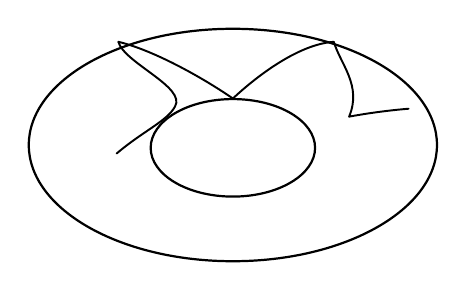
\begin{tikzpicture}[scale=0.72, line cap=round, line join=round]
  \draw[line width=0.8pt] (0,0) ellipse (3.6 and 2.05);
  \draw[line width=0.8pt] (0,-0.05) ellipse (1.45 and 0.86);
  \draw[line width=0.7pt]
    (-2.05,-0.15) .. controls (-1.58,0.25) and (-1.16,0.42) .. (-1.02,0.68)
    .. controls (-0.82,1.02) and (-1.92,1.45) .. (-2.02,1.82)
    .. controls (-1.42,1.68) and (-0.55,1.20) .. (0.00,0.82)
    .. controls (0.46,1.25) and (1.18,1.78) .. (1.78,1.82)
    .. controls (1.90,1.42) and (2.28,1.05) .. (2.05,0.50)
    .. controls (2.48,0.58) and (2.86,0.62) .. (3.10,0.64);
\end{tikzpicture}
\end{center}

In the case of the ellipsoid, the plane of $xy$ being as usual horizontal, and the
equation being
\[
\frac{x^2}{a^2} + \frac{y^2}{b^2} + \frac{z^2}{c^2} = 1,
\]
then if $\lambda$ be the given constant inclination, the boundaries are the series of points
at which the inclination of the normal to the axes of $z$ is $= \lambda$; that is, we have
\[
\frac{z^2}{c^4}
=\left(\frac{x^2}{a^4}+\frac{y^2}{b^4}+\frac{z^2}{c^4}\right)\cos^2\lambda,
\]
or, what is the same thing,
\[
\left(\frac{x^2}{a^4}+\frac{y^2}{b^4}\right)\cos^2\lambda-\frac{z^2}{c^4}\sin^2\lambda=0,
\]
the boundaries are thus two detached ovals, meeting the principal sections $x=0$, $y=0$,
in the points given by
\[
\frac{z}{y}=\pm\frac{c^2}{b^2}\cot\lambda;\qquad
\frac{z}{x}=\pm\frac{c^2}{a^2}\cot\lambda,
\]
and the general form is thus at once perceived.

\medskip
\noindent
12.\ \textit{To every point of space there corresponds a plane, viz.\ considering the several
points as belonging to a solid body which is infinitesimally displaced in any manner,
the plane which corresponds to a point is the plane drawn through the point at right
angles to the direction of the motion; determine the plane which corresponds to a given
point; and connect the result with any general geometrical theory.}

\medskip
The displacements, in the directions of the axes, of a point whose coordinates are
$(x, y, z)$ are given by the ordinary formulae
\begin{align*}
\delta x &= a + q z - r y, \\
\delta y &= b + r x - p z, \\
\delta z &= c + p y - q x,
\end{align*}

\clearpage

\bigskip
\textit{p.~454 [531]}
\smallskip

\noindent
where $a$, $b$, $c$, $p$, $q$, $r$ are constants which determine the particular displacement; hence if $X$, $Y$, $Z$ are current coordinates, the plane corresponding to the point $(x, y, z)$ is
the plane through this point at right angles to the line
\[
\frac{X-x}{\delta x}=\frac{Y-y}{\delta y}=\frac{Z-z}{\delta z},
\]
viz.\ it is the plane
\[
(X - x) (a + qz - ry) + (Y - y) (b + rx - pz) + (Z - z) (c + py - qx) = 0,
\]
or, substituting for $\delta x$, $\delta y$, $\delta z$ their values, reducing and arranging, this is
\begin{align*}
&\quad X(a - r y + q z) \\
&\quad + Y(b - p z + r x) \\
&\quad + Z(c - q x + p y) \\
&\quad +(-ax-by-cz\ .)=0,
\end{align*}
that is, the equation of the plane corresponding to the point $(x, y, z)$ is an equation
linear in regard to the coordinates $(x, y, z)$ of this point; and such that arranging as
above in the form of a square, the coefficients which are symmetrically situate in
regard to the dexter diagonal are equal and of opposite signs, or say that the
coefficients form a skew symmetrical matrix.

More generally, corresponding to the point $(x, y, z)$ we may have the plane
\[
AX + BY + CZ + D = 0,
\]
where $A$, $B$, $C$, $D$ are any linear functions whatever ($= ax + by + cz + d$, etc.) of the
coordinates $(x, y, z)$; this is the general relation which is put in the analytical basis of the
theory of duality; it is in fact (apart from a variable point situate as a
line or a plane, etc.) the general one, to a given point there corresponds a
plane not in general passing through the point; the case above considered is distinguished by the circumstance that for any point whatever the corresponding plane does
pass through the point.

\medskip
\noindent
13.\ \textit{Write down the Lagrangian equations of motion, explaining the notation, and
mode of applying them; and by way of illustration deduce the equations of motion of
three particles, connected so as to form an equilateral triangle (of variable magnitude),
moving in a plane under the action of any forces.}

\medskip
The Lagrangian equations of motion are
\[
\frac{d}{dt}\frac{dT}{d\xi'}-\frac{dT}{d\xi}=\frac{dU}{d\xi},
\]
\[
\frac{d}{dt}\frac{dT}{d\eta'}-\frac{dT}{d\eta}=\frac{dU}{d\eta},
\]
\&c.,

\clearpage

\bigskip
\textit{p.~455 [531]}
\smallskip

\noindent
$\xi$, $\eta$, \ldots\ are here any independent coordinates (in the most general sense of the word)
which serve to determine the position of the system at the time $t$; $T$ is the \textit{vis viva}
function, or half-sum of the mass of each particle of the system into the square of
its velocity, expressed in terms of the coordinates $\xi$, $\eta$, \ldots\ and of their differential
coefficients $\xi'=\dfrac{d\xi}{dt}$, $\eta'=\dfrac{d\eta}{dt}$, \&c.; $T$ is thus a given function of
$\xi,\eta,\ldots,\xi',\eta',\ldots$, homogeneous of the second order as regards the
quantities $\xi'$, $\eta'$, \ldots. The partial differential coefficients of $T$ in regard to
$\xi,\eta,\ldots,\xi',\eta',\ldots$ are thus given functions of $\xi,\eta,\ldots,\xi',\eta',\ldots$;
$U$ is the force-function or sum
\[
\sum m\int(X\,dx+Y\,dy+Z\,dz)
\]
(it being assumed that $Xdx+Ydy+Zdz$ is a complete differential, that is, that there
exists a force-function $U$) expressed in terms of the coordinates $\xi$, $\eta$, \ldots\ and being
thus a given function of these coordinates. The terms $\dfrac{d}{dt}\dfrac{dT}{d\xi'}$, \&c.,
contain, it is clear, (and that linearly) the second differential coefficients
$\xi''=\dfrac{d^2\xi}{dt^2}$, \&c.; the equations thus establish between the coordinates
$\xi,\eta,\ldots$ and their first and second differential coefficients in regard to the time
a system of relations, the number of which is equal to that of the coordinates, and
which therefore would by integration lead to the expression of the coordinates
$\xi,\eta,\ldots$ in terms of the time.

It has been tacitly assumed that $T$, $U$ were functions of $\xi,\eta,\ldots,\xi',\eta',\ldots$,
and of $\xi,\eta,\ldots$, not containing the time $t$; this is the ordinary case, but there are
cases in which $T$ and $U$ or either of them may also contain the time $t$.

In the proposed case of the three particles, if $m_1$, $m_2$, $m_3$ be their masses, $r$ the
side of the equilateral triangle, $x$, $y$ the coordinates of $m_1$, $\theta$, $\theta+60^\circ$
(or write for convenience $\theta+a$) the inclinations of $m_1m_2$, $m_1m_3$ to the axis of $x$,
then the coordinates of $m_2$, $m_3$ will be
\[
x+r\cos\theta,\quad x+r\cos(\theta+a),
\]
\[
y+r\sin\theta,\quad y+r\sin(\theta+a).
\]

We have
\begin{align*}
T &= \tfrac12 m_1(x'^2+y'^2)\\
&\quad+\tfrac12 m_2[(x'+r'\cos\theta-r\sin\theta\,\theta')^2
 +(y'+r'\sin\theta+r\cos\theta\,\theta')^2]\\
&\quad+\tfrac12 m_3[\{x'+r'\cos(\theta+a)-r\sin(\theta+a)\theta'\}^2
 +\{y'+r'\sin(\theta+a)+r\cos(\theta+a)\theta'\}^2]\\
&=\tfrac12(m_1+m_2+m_3)(x'^2+y'^2)\\
&\quad+m_2[x'(r'\cos\theta-r\sin\theta\,\theta')+
y'(r'\sin\theta+r\cos\theta\,\theta')]\\
&\quad+m_3[x'\{r'\cos(\theta+a)-r\sin(\theta+a)\theta'\}
+y'\{r'\sin(\theta+a)+r\cos(\theta+a)\theta'\}]\\
&\quad+\tfrac12(m_2+m_3)(r'^2+r^2\theta'^2),
\end{align*}

\clearpage

\bigskip
\textit{p.~456 [531]}
\smallskip

\noindent
a given function of $x$, $y$, $r$, $\theta$, $x'$, $y'$, $r'$, $\theta'$; also
\[
U=m_1\int(Xdx+Ydy)+\&c.
\]
will be a given function of $x$, $y$, $r$, $\theta$; and the equations of motion will be
\begin{align*}
\frac{d}{dt}\frac{dT}{dx'}-\frac{dT}{dx} &= \frac{dU}{dx},\\
\frac{d}{dt}\frac{dT}{dy'}-\frac{dT}{dy} &= \frac{dU}{dy},\\
\frac{d}{dt}\frac{dT}{dr'}-\frac{dT}{dr} &= \frac{dU}{dr},\\
\frac{d}{dt}\frac{dT}{d\theta'}-\frac{dT}{d\theta} &= \frac{dU}{d\theta}.
\end{align*}

\medskip
\noindent
14.\ \textit{From the integrals $x = a\cos t + a'\sin t$, $y = b\cos t + b'\sin t$, of the dynamical
equations $\dfrac{d^2x}{dt^2} = -x$, $\dfrac{d^2y}{dt^2} = -y$, derive a simultaneous solution of the two partial differential
equations
\[
\frac{dS}{dt}+\frac12\left\{\left(\frac{dS}{dx}\right)^2+\left(\frac{dS}{dy}\right)^2\right\}
=-\frac12(x^2+y^2),
\]
\[
\frac{dS}{dt}+\frac12\left\{\left(\frac{dS}{da}\right)^2+\left(\frac{dS}{db}\right)^2\right\}
=-\frac12(a^2+b^2).
\]}

\medskip
Writing $U=-\tfrac12(x^2+y^2)$, we have
\begin{align*}
x &= a\cos t + a'\sin t,\\
y &= b\cos t + b'\sin t,
\end{align*}
as the integrals of the equations of motion
\[
\frac{d^2x}{dt^2}=\frac{dU}{dx}, \quad \frac{d^2y}{dt^2}=\frac{dU}{dy};
\]
moreover
\[
x' = -a\sin t + a'\cos t,
\]
\[
y' = -b\sin t + b'\cos t,
\]
where $a$, $b$, $a'$, $b'$ are the initial values of $x$, $y$, $x'$, $y'$ respectively $\left(x' = \dfrac{dx}{dt}, y' = \dfrac{dy}{dt}\right)$.

Hence the Principal Function
\[
S = \int_0^t \tfrac{1}{2}(T + U) \dd t
\]
\[
= \tfrac{1}{2}\int_0^t (x'^2 + y'^2 - x^2 - y^2)\,dt,
\]
expressed as a function of $x$, $y$, $a$, $b$, $t$, will satisfy simultaneously the proposed partial
differential equations.

We have
\[
x'^2 + y'^2 - x^2 - y^2 = (a'^2+b'^2-a^2-b^2)\cos 2t-2(aa'+bb')\sin 2t.
\]

\clearpage

\bigskip
\textit{p.~457 [531]}
\smallskip

Hence
\[
4S = \tfrac{1}{2}(a'^2 + b'^2 - a^2 - b^2)\sin 2t + 2(aa' + bb')(1 - \cos 2t)
\]
\[
= (a'^2+b'^2)\sin 2t-(a^2+b^2)\sin 2t-4(aa'+bb')\sin^2 t.
\]

But
\[
a'\sin t=x-a\cos t,
\]
\[
b'\sin t=y-b\cos t.
\]
Hence
\[
(aa'+bb')\sin t=ax+by-(a^2+b^2)\cos t,
\]
\[
(a'^2+b'^2)\sin^2 t=x^2+y^2-2(ax+by)\cos t+(a^2+b^2)\cos^2 t,
\]
and substituting these values
\[
4S=\frac{2\sin t\cos t}{\sin^2 t}
\{x^2+y^2-2(ax+by)\cos t+(a^2+b^2)\cos^2 t\}
\]
\[
\quad -(a^2+b^2)\,2\sin t\cos t
\]
\[
\quad -4\sin t\{ax+by-(a^2+b^2)\cos t\}
\]
\[
=2(x^2+y^2)\frac{\cos t}{\sin t}
-\frac{4}{\sin t}(ax+by)+2(a^2+b^2)\frac{\cos t}{\sin t};
\]
or, what is the same thing,
\[
S=\tfrac12(x^2+y^2+a^2+b^2)\cot t-2(ax+by)\cosec t,
\]
which value of $S$ satisfies the two partial differential equations.

More generally, the two equations are satisfied by
\[
S=c+\text{foregoing value},
\]
($c$ an arbitrary constant) which new value, considered as a solution of the first equation,
contains the three arbitrary constants $c$, $a$, $b$, and is thus a \textit{complete} solution; and
similarly considered as a solution of the second equation, it contains the three arbitrary
constants $c$, $x$, $y$, and is thus a \textit{complete} solution.

I venture to add a few remarks in illustration of what is required in the papers
sent up in an Examination.

In the latter part of question (2) (form of the equation for a system of parallel
curves) it is worse than useless to say
$\dfrac{df}{dc}\div\left\{\left(\dfrac{df}{dx}\right)^2+\left(\dfrac{df}{dy}\right)^2\right\}^{1/2}$
[p.~441] must be constant:
a good and sufficient answer would be that it must be constant in virtue of the given
equation $f(x,y,c)=0$. So in question (13) (the Lagrangian equations of motion), it is
quite essential to explain [p.~455] that $T$, $U$ are given functions of
$\xi,\eta,\ldots,\xi',\eta',\ldots$ and of $\xi,\eta,\ldots$ respectively; but for this the equations
might be partial differential equations for the determination of $T$, $U$, or nobody knows what:
it is natural and proper to explain further that $T$ is homogeneous of the second order in
regard to the derived functions $\xi'$, $\eta'$, \ldots. In question (14) the answer [p.~456] that
$S=\frac12\int_0^t(x'^2+y'^2-x^2-y^2)\,dt$ expressed as a function of $x,y,a,b,t$ will satisfy
simultaneously the proposed equations---would be, not of course a complete answer, but a
good and creditable one; without the words ``expressed as a function of $x,y,a,b,t$'' it would
be altogether worthless. A clear and precise indication of a process of solution is very much better than a
detailed solution incorrectly worked out.

\hfill C.\ VIII.\hspace{2em} 58

\clearpage

% ============================================================
% PAPER 532
% Note on the Integration of Certain Differential Equations by Series
% Book pages 458--462
% ============================================================
\section{[532]}
\subsection{Note on the Integration of Certain Differential Equations by Series.}

\begin{center}
\textit{[From the Oxford, Cambridge, and Dublin Messenger of Mathematics, vol.~\textsc{v}.\ (1869), pp.~77--82.]}
\end{center}

\textsc{There} is a speciality in the integration of certain differential equations by
series, which (though evidently quite familiar to those who have written on the
subject---Ellis, Boole, Hargreave) has not, it appears to me, been exhibited in the
clearest form. To fix the ideas, consider a linear differential equation of the second
order integrable in the form $y=Ax^\lambda+Bx^{\lambda+1}+\ldots$; $\lambda$ is determined by a quadratic
equation, and for each value of $\lambda$ the coefficients $B$, $C$, \ldots\ are given multiples of $A$;
we have thus the general solution
\[
y=A\left(x^\alpha+\frac{B}{A}x^{\alpha+1}\ldots\right)
+K\left(x^\beta+\frac{L}{K}x^{\beta+1}+\&c.\ldots\right).
\]

The speciality referred to is, when the two roots differ by an integer number;
suppose $\alpha$ is the smaller root, and $\beta=\alpha+k$ ($k$ a positive integer) the larger. Then,
inasmuch as the series
\[
y=Ax^\alpha+Bx^{\alpha+1}+\&c.
\]
is identical in form with the general solution as above written down, it is clear that,
starting with the root $\lambda=\alpha$, the coefficients beginning with that of $x^\beta$, $=x^{\alpha+k}$, ought
not to be any longer determinate multiples of $A$, but should contain a new arbitrary
constant $K$, and thus that the series derived from the root $\lambda=\alpha$ should be the
general solution containing two arbitrary constants. The most simple case is when
the substitution of the series in the differential equation leads to a relation between
two consecutive coefficients of the series. Here the values $\frac BA$, $\frac CA$, \&c.\ are fractions

\clearpage

\bigskip
\textit{p.~459 [532]}
\smallskip

the numerators and denominators of which are factorial functions of $\alpha$ such that, for
some coefficient $\frac FA$ preceding $\frac KA$ (if $K$ is the coefficient of $x^{\alpha+k}$), and for all the
succeeding coefficients $\frac GA$, \&c.\ there is in the numerators one and the same evanescent
factor; this being so, it is allowable to write $F=0$, $G=0$, \&c.\ giving for the
differential equation the finite solution
\[
y=A\left(x^\alpha+\frac BAx^{\alpha+1}\ldots+\frac EAx^{\alpha+e}\right);
\]
but, if notwithstanding the evanescent factor, we carry on the series, then in the
coefficient of $x^{\alpha+k}$ there occurs in the denominator the same evanescent factor, so
that the coefficient of this term presents itself in the form $A\frac PQ\cdot\frac00$, $=$ an arbitrary
constant $K$ (since the $\frac00$ is essentially indeterminate), and the solution is thus
obtained is the form
\[
y=A\left(x^\alpha+\frac BAx^{\alpha+1}\ldots+\frac EAx^{\alpha+e}\right)
+K\left(x^{\alpha+k}+\frac LKx^{\alpha+k+1}+\&c.\right),
\]
viz.\ there is one particular solution which is finite.

Take for example the equation
\[
\frac{d^2y}{dx^2}+q\frac{dy}{dx}-\frac{2}{x^2}y=0 \tag{I},
\]
mentioned Cambridge Math.\ Journal, t.~\textsc{ii.}\ p.~176 (1840).\ If the integral is assumed to
be
\[
y = Ax^\alpha + Bx^{\alpha+1} + Cx^{\alpha+2} + \&c.,
\]
then we find
\begin{align*}
(\alpha+1)(\alpha-2)A&=0,\\
(\alpha-1)(\alpha+2)B+q\alpha A&=0,\\
\alpha(\alpha+3)C+q(\alpha+1)B&=0,\\
(\alpha+1)(\alpha+4)D+q(\alpha+2)C&=0,\\
\&c.
\end{align*}

Hence $\alpha=-1$, or else $\alpha=2$;
\begin{align*}
B&=\frac{-q\alpha}{(\alpha-1)(\alpha+2)}A,\\
C&=\frac{q^2\alpha(\alpha+1)}{(\alpha-1)\alpha(\alpha+2)(\alpha+3)}A,\\
D&=\frac{-q^3\alpha(\alpha+1)(\alpha+2)}{(\alpha-1)\alpha(\alpha+1)(\alpha+2)(\alpha+3)(\alpha+4)}A,\\
\&c.
\end{align*}

\hfill 58---2

\clearpage

\bigskip
\textit{p.~460 [532]}
\smallskip

Here taking $\alpha = -1$, we are at liberty to make $C$ and all the following coefficients
$=0$; in fact, if we commence by assuming
\[
y = Ax^\alpha + Bx^{\alpha+1},
\]
the equations
\begin{align*}
(\alpha+1)(\alpha-2)A&=0,\\
(\alpha-1)(\alpha+2)B+q\alpha A&=0,\\
q(\alpha+1)B&=0,
\&c.
\end{align*}
are all satisfied if only $\alpha=-1$,
$B=\dfrac{-q\alpha A}{(\alpha-1)(\alpha+2)}$; and we have thus the finite
solution $y=A\left(\dfrac1x-\dfrac q2\right)$; but if we continue the series, retaining $D$ to represent the
indeterminate quantity
$\dfrac{-q^3\alpha(\alpha+1)(\alpha+2)}{(\alpha-1)\alpha(\alpha+1)(\alpha+2)(\alpha+3)(\alpha+4)}A$, we have the solution
\[
y=A\left(\frac1x-\frac12 q\right)+D\left(x^2-\frac12 qx^3+\&c.\right),
\]
the second member of which is in fact the series derived from the root $\alpha=2$.
This series is expressible by means of an exponential, viz.\ we have
\[
x^2-\tfrac12 qx^3+\&c.=\frac{12}{q^3}\left\{\left(\frac1x+\tfrac12q\right)e^{-qx}
-\left(\frac1x-\tfrac12q\right)\right\},
\]
and the complete integral is thus
\[
y=A\left(\frac1x-\tfrac12q\right)+B\left(\frac1x+\tfrac12q\right)e^{-qx},
\]
but this result is not immediately connected with the investigation. It may however
be noticed that, writing $z=ye^{qx}$, the equation in $z$ is
\[
\frac{d^2z}{dx^2}-q\frac{dz}{dx}-\frac{2}{x^2}z=0,
\]
which only differs from the original equation in that it has $-q$ in place of $q$:
there is consequently the particular solution $z=\dfrac1x+\tfrac12q$, giving for $y$ the particular
solution $y=\left(\dfrac1x+\tfrac12q\right)e^{-qx}$, and we have thence the complete solution as above.

Consider, secondly, the differential equation
\[
\frac{d^2y}{dx^2}-\left(\frac14q^2+\frac{2}{x^2}\right)y=0 \tag{II},
\]
(derived from the equation (I) by writing therein $ye^{-qx}$ in place of $y$); this equation
is satisfied by the series
\[
y=Ax^\alpha+Bx^{\alpha+2}+Cx^{\alpha+4}+\&c.
\]

\clearpage

\bigskip
\textit{p.~461 [532]}
\smallskip

Then $\alpha=-1$ or $\alpha=+2$, but here the series belonging to $\alpha=-1$ contains only odd
powers, the other contains only even powers of $x$; hence the two series do not
coalesce as in the former case, and the first series is obtained without the indeterminate symbol $\dfrac{0}{0}$ in any of the coefficients. We have in fact
\begin{align*}
(\alpha+1)(\alpha-2)A&=0,\\
(\alpha+3)\alpha B-\tfrac14q^2A&=0,\\
(\alpha+5)(\alpha+2)C-\tfrac14q^2B&=0,\\
\&c.
\end{align*}
and there is not, in the series in question for the value of $\alpha = -1$ (or other series) any evanescent
factor, either in the numerator or in the denominators.

But consider, thirdly, the differential equation
\[
\frac{d^2y}{dx^2}+(q-2\theta)\frac{dy}{dx}
+\left(\theta^2-q\theta-\frac{2}{x^2}\right)y=0 \tag{III},
\]
(derived from (I) by writing therein $ye^{-\theta x}$ in place of $y$). This is satisfied by the series
\[
y = Ax^\alpha + Bx^{\alpha+1} + Cx^{\alpha+2} + Dx^{\alpha+3} + \&c.,
\]
where $\alpha=-1$ or $\alpha=+2$ as before; in the series belonging to $\alpha=-1$, the coefficient
$D$ should become indeterminate. The relation between the coefficients is here a
relation between three consecutive coefficients, viz.\ we have
\begin{align*}
(\alpha+1)(\alpha-2)A&=0,\\
(\alpha+2)(\alpha-1)B+(q-2\theta)\alpha A&=0,\\
(\alpha+3)\alpha C+(q-2\theta)(\alpha+1)B+(\theta^2-q\theta)A&=0,\\
(\alpha+4)(\alpha+1)D+(q-2\theta)(\alpha+2)C+(\theta^2-q\theta)B&=0,\\
(\alpha+5)(\alpha+2)E+(q-2\theta)(\alpha+3)D+(\theta^2-q\theta)C&=0,\\
\&c.
\end{align*}
It is to be shown that in the series for $\alpha=-1$, the expression
$(q-2\theta)(\alpha+2)C+(\theta^2-q\theta)B$ contains the evanescent factor $(\alpha+1)$,
and consequently that $D$ is indeterminate; we have in fact
\[
B=-\frac{(q-2\theta)\alpha}{(\alpha+2)(\alpha-1)}A,
\]
and thence
\[
C=\frac{1}{\alpha(\alpha+3)}
\left\{\frac{(q-2\theta)^2\alpha(\alpha+1)}{(\alpha+2)(\alpha-1)}
-(\theta^2-q\theta)\right\}A,
\]
\[
(q-2\theta)(\alpha+2)C+(\theta^2-q\theta)B
\]

\clearpage

\bigskip
\textit{p.~462 [532]}
\smallskip

and then, after reduction, the remaining multiplier is
\[
-\frac{\alpha+2}{\alpha(\alpha+3)}
+\frac{\alpha}{(\alpha+2)(\alpha-1)}
=\frac{2\alpha^3+6\alpha^2-4}{(\alpha-1)\alpha(\alpha+2)(\alpha+3)}
=\frac{2(\alpha+1)(\alpha^2+2\alpha-2)}{(\alpha-1)\alpha(\alpha+2)(\alpha+3)},
\]
so that the whole expression contains the factor $\alpha + 1$. But observe that in the
present case, if (as is allowable) we write $D=0$, the next coefficient $E$ (depending
not on $D$ only, but on $D$ and $C$) will not vanish; so that the solution obtained on
the assumption $D=0$ will go on to infinity: and if instead of assuming $D=0$, we
assume $D=$ an arbitrary quantity $D'$, then $E$ and the subsequent coefficients will
contain terms depending on $D'$, and the complete form of the series belonging to
$\alpha = -1$ will be
\[
y=A\left(x^{-1}+\frac BA+\frac CAx+\frac DAx^2+\frac EAx^3+\&c.\right)
+D'\left(x^2+\frac{E'}{D'}x^3+\&c.\right),
\]
where the second member is in fact the series belonging to $\alpha=2$. It is hardly
necessary to remark that the solution thus obtained can be expressed by means of
exponentials, viz.\ that the solution is
\[
y=A\left(\frac1x-\tfrac12q\right)e^{\theta x}
+D'\frac{12}{q^3}
\left\{\left(\frac1x+\tfrac12q\right)e^{-qx}
-\left(\frac1x-\tfrac12q\right)\right\}e^{\theta x}.
\]

\clearpage

% ============================================================
% PAPER 533
% On the Binomial Theorem, Factorials, and Derivations
% Book pages 463--466
% ============================================================
\section{[533]}
\subsection{On the Binomial Theorem, Factorials, and Derivations.}

\begin{center}
\textit{[From the Oxford, Cambridge, and Dublin Messenger of Mathematics, vol.~\textsc{v}.\ (1869), pp.~102--114.]}
\end{center}

\textsc{The} following was part of my course of lectures in the year 1867.

The proof commonly called ``Euler's'' of the binomial theorem is as follows: the
theorem is assumed to be true for positive integer indices; that is, it is assumed that
for any positive integer $m$ we have
\[
(1 + x)^m = 1 + mx + \frac{m(m-1)}{1\cdot 2}x^2 + \&c.
\]
This being so, since $(1 + x)^m \cdot (1 + x)^n = (1 + x)^{m+n}$, the equation
\[
\left[1 + mx + \frac{m(m-1)}{1\cdot 2}x^2 + \&c.\right]\cdot\left[1 + nx + \frac{n(n-1)}{1\cdot 2}x^2 + \&c.\right]
\]
\[
\quad = 1 + (m + n)x + \frac{(m + n)(m + n - 1)}{1\cdot 2}x^2 + \&c.
\]
is true for any positive integer values whatever of $m$ and $n$; the equation is therefore
true identically; and it is consequently true for all values whatever of $m$ and $n$.
But any function $\phi_m$ of $m$, satisfying the functional equation
$\phi_m\phi_n=\phi_{m+n}$, is an $m$th power, $=C^m$ suppose; that is, we have
\[
C^m = 1 + mx + \frac{m(m-1)}{1\cdot 2}x^2 + \&c.
\]
where $C$ is a constant; viz.\ it is independent of $m$; but the value of $C$ will of course depend upon $x$; and if, in order to determine it, we write $m=1$, the equation gives
$C=1+x$; that is, we have
\[
(1 + x)^m = 1 + mx + \frac{m(m-1)}{1\cdot 2}x^2 + \&c.,
\]
which is the binomial theorem in its general form.

\clearpage

\bigskip
\textit{p.~464 [533]}
\smallskip

It is to be observed that there is not in the demonstration any employment of
the so called ``principle of equivalent forms,'' we do not from the truth of an equation
for positive integer values of $m$, $n$, infer the truth of it for any values whatever of
$m$, $n$; there is the intermediate step, that being true for the integers, it is true identically,
and the identical truth of the equation depends on the circumstance that comparing
on the two sides of the equation the coefficients of the successive powers $x$, $x^2$, $x^3$, \&c.,
these coefficients are in every case finite, rational, and integral functions of $m$, $n$.

For instance, comparing the coefficients of $x^2$, we have
\[
(m+n)(m+n-1)=m(m-1)+2mn+n(n-1),
\]
and any such equation, being true for all positive integer values of $m$, $n$, will be
true identically; developing the two sides, the equation is in fact
\[
m^2+2mn+n^2-m-n=m^2-m+2mn+n^2-n.
\]
The reasoning is thus perfectly good; but I remark that it is quite as easy to prove
the general equation of which the last mentioned equation is an example, as it is to
prove the binomial theorem for positive integer indices; and consequently that we can
without the aid of the binomial theorem for positive integer indices prove the fundamental
equation
\[
(1 + x)^{m+n} = (1 + x)^m (1 + x)^n
\]
To show this I introduce the factorial notation and it is readily found to
be
\[
m(m-1)\cdots(m-r+1)=[m]^r;
\]
this being so, the equation obtained by comparing the coefficients of $x^r$ is readily found
to be
\[
[m+n]^r=[m]^r+r[m]^{r-1}[n]^1+\frac{r(r-1)}{1\cdot2}[m]^{r-2}[n]^2+\&c.,
\]
and I say that, this, the \textit{factorial binomial theorem for a positive integer index $r$},
is proved as easily and in the same manner as the binomial theorem for a like value
of the index; or say in equation
\[
(m + n)^r = m^r + rm^{r-1}\cdot n + \frac{r(r-1)}{1\cdot 2}m^{r-2}\cdot n^2 + \&c.
\]
To show how this is, I form the values of $[m+n]^1$, $[m+n]^2$, $[m+n]^3$, \&c.\ successively,
by what may be termed the process of varied multiplication: we have
\[
[m + n]^1 = m + n.
\]

\clearpage

\bigskip
\textit{p.~465 [533]}
\smallskip

\noindent
to obtain $[m+n]^2$ we have to multiply this by $m+n-1$: in regard to the first term
$m$, I write the multiplier under the form $(m-1)+n$, and in regard to the second
term $n$, under the form $m + (n - 1)$; the process then stands
\[
\begin{array}{rcc}
[m+n]^1&=&m+n\\
m+n-1&=&(m-1)+n\quad;\quad m+(n-1)\\ \hline
[m+n]^2&=&m(m-1)+mn+mn+n(n-1)\\
&=&[m]^2+2[m]^1[n]^1+[n]^2.
\end{array}
\]

To form $[m + n]^3$ we have to multiply by $m + n - 2$; in regard to the first term, this
is written under the form $(m - 2) + n$; in regard to the second term under the form
$(m - 1) + (n - 1)$; and in regard to the third term under the form $m + (n - 2)$; the
product is thus obtained in the form
\[
[m]^3+[m]^2[n]^1+2[m]^2[n]^1+2[m]^1[n]^2+[m]^1[n]^2+[n]^3
\]
\[
=[m]^3+3[m]^2[n]^1+3[m]^1[n]^2+[n]^3;
\]
and so on; the law of the terms is obvious; and the numerical coefficients are in
effect obtained as follows:
\[
\begin{array}{ccccc}
& & 1, & & \\
& 1, & & 1, & \\
& & 1, & 1, & 1, \\
1, & 1, & & & \\
& 1, & 2, & 1, & 1, \\
& & 1, & 2, & 1, \\
1, & 3, & 3, & 1, & \\
\&c.
\end{array}
\]
viz.\ by precisely the same process as is used in finding the numerical coefficients in
the powers $(m + n)^1$, $(m + n)^2$, $(m + n)^3$, \&c.; and we thus see that for any integer value
$r$ of the index, we have a factorial binomial theorem, wherein the numerical coefficients
are the same as in the binomial theorem for the same index.

\clearpage

\bigskip
\textit{p.~466 [533]}
\smallskip

But the method of varied multiplication may be applied to the demonstration of
a much more general theorem; viz.\ we may use it to develope a product such as
\[
(h-a)(h-b)(h-c)(h-d)(h-e),
\]
according to a series of products
\[
(h-\alpha)(h-\beta)(h-\gamma)(h-\delta)(h-\epsilon),
\]
\[
(h-\alpha)(h-\beta)(h-\gamma)(h-\delta),
\]
\[
(h-\alpha)(h-\beta)(h-\gamma),
\]
\[
(h-\alpha)(h-\beta),
\]
\[
(h-\alpha),
\]
\[
1.
\]

For this purpose, starting with
\[
h-a=h-\alpha+\alpha-a,
\]
we multiply by $h-b$, written first under the form $h-\beta+\beta-b$, and then under the
form $h-\alpha+(\alpha-b)$; we have thus
\[
\begin{aligned}
(h-a)(h-b)={}&(h-\alpha)(h-\beta)\\
&+(h-\alpha)\{(\alpha-a)+(\beta-b)\}\\
&+1\cdot(\alpha-a)(\alpha-b),
\end{aligned}
\]
and so on. It is easy to see that we may for instance write
\[
\begin{aligned}
(h-a)(h-b)(h-c)(h-d)(h-e)
={}&(h-\alpha)(h-\beta)(h-\gamma)(h-\delta)(h-\epsilon)\\
&+(h-\alpha)(h-\beta)(h-\gamma)(h-\delta)
\left(\begin{array}{c}
\alpha,\beta,\gamma,\delta,\epsilon\\
a,b,c,d,e
\end{array}\right)_1\\
&+(h-\alpha)(h-\beta)(h-\gamma)
\left(\begin{array}{c}
\alpha,\beta,\gamma,\delta\\
a,b,c,d,e
\end{array}\right)_2\\
&+(h-\alpha)(h-\beta)
\left(\begin{array}{c}
\alpha,\beta,\gamma\\
a,b,c,d,e
\end{array}\right)_3\\
&+(h-\alpha)
\left(\begin{array}{c}
\alpha,\beta\\
a,b,c,d,e
\end{array}\right)_4\\
&+1\left(\begin{array}{c}
\alpha\\
a,b,c,d,e
\end{array}\right)_5 .
\end{aligned}
\]

\clearpage

\end{document}
